\documentclass[10pt]{article}
\usepackage{amsmath}
\usepackage{listings}
\usepackage{graphicx}
\usepackage{float}
\usepackage{tabularx}
\graphicspath{ {./images/} }
\begin{document}
{\centering
    CSU44061 Machine Learning - Week 8
    \par
    Samuel Petit - 17333946
    \par
    Code for all questions provided in the appendix.
}
\section*{Question i}
\subsection*{Part a}
In order to do so there are 2 problems to solve:
- knowing how many iterations to apply the kernel within the image (for columns and rows)
- For each iteration, compute the resulting value to place in the output

To do so, I start by computing both:
\begin{equation*}
    rows = \# rows_{image} - \# rows_{kernel} + 1
\end{equation*}
\begin{equation*}
    columns = \# columns_{image} - \# columns_{kernel} + 1
\end{equation*}

Then, given that both $rows$ and $columns$ are positive numbers, we know
the amount of positions to place the kernel within the image on both the x and y axis.

The first step is then to iterate over both ranges, that is:
\begin{lstlisting}
x_positions = len(image) - len(kernel) + 1
y_positions = len(image[0]) - len(kernel[0]) + 1
# Make sure kernel and image sizes are valid
assert x_positions > 0 and y_positions > 0, 
        "image should not be smaller than kernel"
# Iterate over kernel positions within the image
for i in range(x_positions):
    for j in range(y_positions):
        # Compute the output point here
\end{lstlisting}

Let's now look at the second problem to solve, that is, given a certain x and y
iteration (here represented as i and j), compute the resulting value to position
in the output matrix.

To do so, I iterate over the kernel matrix rows and columns such as to compute:

\begin{equation*}
    output_{i,j} = \sum_{k = 0}^{\#kernel_{rows}}\sum_{l = 0}^{\#kernel_{columns}} kernel^{(k,l)} * image^{(i + k, j + l)}
\end{equation*}

That it, for each point in the kernel, we multiply it to its corresponding point (using the offset
of i and j), once we have done so for all kernel points we have the result value for the
point ${i,j}$ of the output matrix.

In code this looks like:
\begin{lstlisting}
sum = 0
for k in range(len(kernel)):
    for l in range(len(kernel[0])):
        sum = sum + (kernel[k][l] * image[i + k][j + l])
\end{lstlisting}

Finally, all we need to do now is use this sum to form the current output row and
finally use the row to build the output matrix. All together:

\begin{lstlisting}
def convolutional_layer(image, kernel):
    x_positions = len(image) - len(kernel) + 1
    y_positions = len(image[0]) - len(kernel[0]) + 1
    assert x_positions > 0 and y_positions > 0, 
            "image should not be smaller than kernel"
    result = []
    for i in range(x_positions):
        row = []
        for j in range(y_positions):
            sum = 0
            for k in range(len(kernel)):
                for l in range(len(kernel[0])):
                    sum = sum + (kernel[k][l] * 
                                image[i + k][j + l])
            row.append(sum)
        result.append(row)
    return result
\end{lstlisting}

\subsection*{Part b}
I chose the picture of a triangle found online:

\begin{center}
    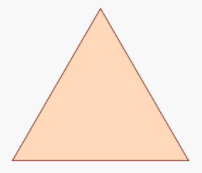
\includegraphics[scale=0.3]{triangle.PNG}
\end{center}

Using the code provided in the assignment and the above picture as an input.
I can apply the 2 provided kernels to my image, we obtain the following
outputs:
\vspace{5mm} %5mm vertical space
Kernel 1:
\begin{center}
    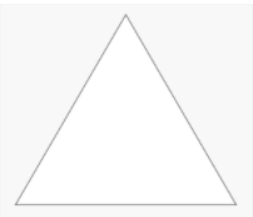
\includegraphics[scale=0.3]{ml_triangle_1.PNG}
\end{center}

\vspace{5mm} %5mm vertical space
Kernel 2:
\begin{center}
    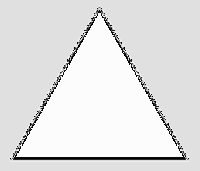
\includegraphics[scale=0.3]{ml_triangle_2.PNG}
\end{center}

\section{Question ii}
\subsection*{Part a}
The downloaded code uses the following ConvNet code:
\begin{lstlisting}
model.add(Conv2D(16, (3,3), padding='same',
        input_shape=x_train.shape[1:],activation='relu'))
model.add(Conv2D(16, (3,3), strides=(2,2), 
                    padding='same', activation='relu'))
model.add(Conv2D(32, (3,3), padding='same', 
                                    activation='relu'))
model.add(Conv2D(32, (3,3), strides=(2,2),
                    padding='same', activation='relu'))
model.add(Dropout(0.5))
model.add(Flatten())
model.add(Dense(num_classes, activation='softmax',
            kernel_regularizer=regularizers.l1(0.0001)))
\end{lstlisting}

We notice a list of sequential steps are added, in order we find:

\begin{itemize}
    \item A 2D Convolution Layer which use 16 filters to learn from. a kernel size of 3x3,
    it also uses padding such as to make outputs the same dimensions as the input, finally
    it also uses 'relu' validation (or rectified linear activation function 
    ) is a method which will map the output to 0 if it is negative.
    \item We then find another 2D Convolution Layer with 16 filters,
    3x3 size, uses padding to keep the same output size and 'relu' activation. The
    difference being that it uses a Stride of size 2x2 such as to downsample
    (it determines how much the window moves by - the default being 1x1)
    \item We then find the exact same 2 steps as we've seen above, in the
    same order with the difference that the filter size is set to 32 instead of 16.
    \item We then find a Droupout step, which sets randomly input values to 0
    with a rate of 0.5 here. This helps to prevent overfitting. It will also
    update non-0 values such as to keep the sum of values consistent.
    \item We then have a Flatten step which simply maps the data to be flat
    \item The final step is a Dense step which is a step for densely connected neural network layers,
    it uses the activation function provided such as to form its output. It uses 10 units (or classes) as specified
    in the downloaded code, L1 regularisation and the activation function is set to
    'softmax' which outputs the values of a probability density function.
\end{itemize}

\subsection*{Part b}
\subsubsection*{Section i}
By simply running the program and reading the output from the
console we find the metrics required by the question:

\begin{itemize}
    \item This model has a total of: 37,146 parameters
    \item The layer with the most parameters is the Dense layer,
    which has 20,490 parameters.
    \item When I ran the code I found that the accuracy on the
    test data was of 0.5, on the train data I obtain an accuracy
    of 0.62. We find that the accuracy does drop by some considerable
    amount compared with the train data ($0.62 - 0.5 = 0.12$), however that makes sense
    as the test data is data the model hasn't seen before, unlike the train.
\end{itemize}

I trained a DummyRegressor model to use as a baseline model for comparison.
This model predicts the most commonly seen value, it is very
straightforward to train:
\begin{lstlisting}
    dummy_model = DummyRegressor().fit(x_train, y_train)
\end{lstlisting}

I then use the same methods as included in the provided code to
obtain an accuracy metric, we find the that baseline model
has an accuracy of 0.1 for both the test and train data. We can 
clearly confirm that our previous model is doing very well in comparison, with an accuracy increase of
$0.5 - 0.1 = 0.4$ on the test data and $0.62 - 0.1 = 0.52$ on the test data.

\subsubsection{Section ii}
The graph we obtain the history variable in the provided code is the following:

\begin{center}
    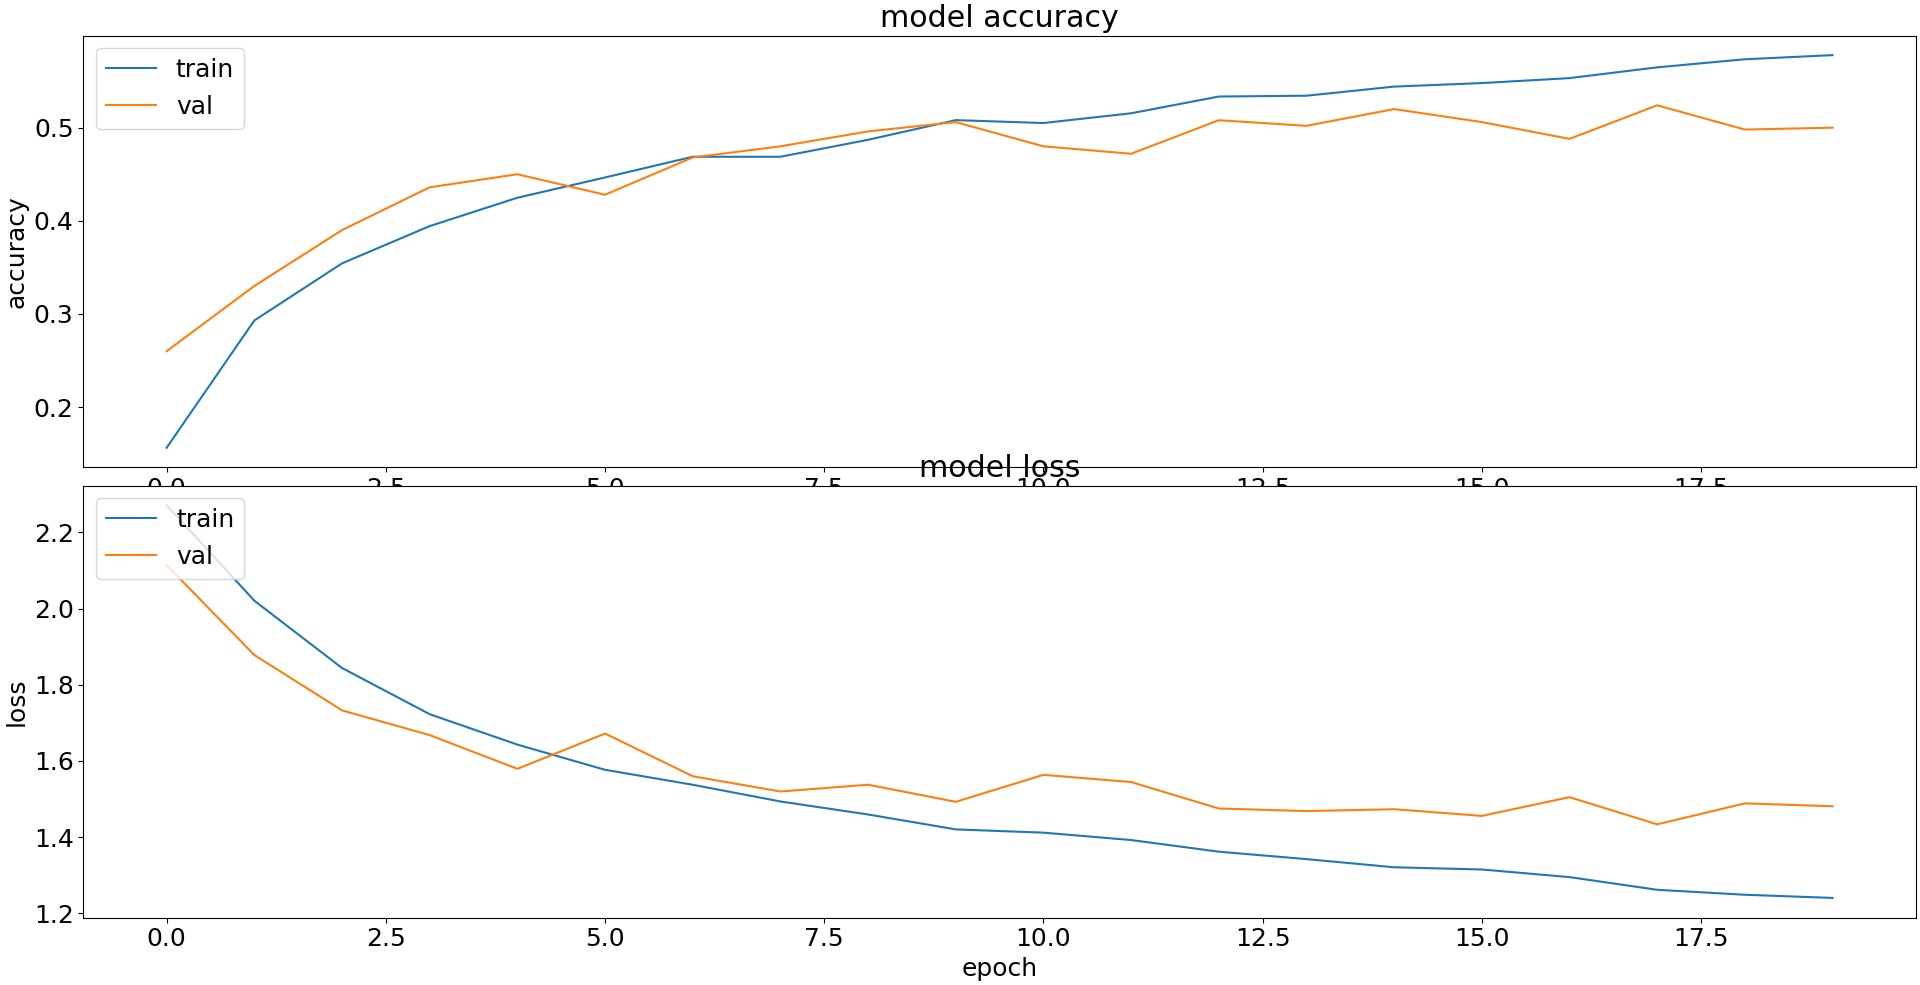
\includegraphics[scale=0.3]{default_5k.png}
\end{center}

\section*{Appendix}


\end{document}
